\documentclass[10pt]{beamer}
\usetheme{metropolis}
% all imports
\usepackage[utf8]{inputenc}
\usepackage{lmodern}
\usepackage[T1]{fontenc}
\usepackage{appendixnumberbeamer}
\usepackage{hyperref}
\usepackage{booktabs}
\usepackage{bm}
\usepackage[scale=2]{ccicons}
\usepackage[cache=false]{minted}
\usepackage{pgfplots}
\usepackage{array,colortbl,xcolor}
\usepgfplotslibrary{dateplot}
\usepackage{setspace}
\usepackage{etoolbox}
\usepackage{xspace}
\usepackage{tikz}
\usetikzlibrary{shapes,arrows,positioning,fit,backgrounds}
\usepackage{tkz-euclide}

\AtBeginEnvironment{quote}{\singlespacing}


\AtBeginEnvironment{quote}{\singlespacing}

% new commands
\input{all_new_commands}

% definitions
\input{definitions/colors}
% Tikzstyles for Computation Graphs

% nodes
\tikzstyle{noop} = [circle, draw=none, fill=red, minimum size = 10pt]
\tikzstyle{op} = [circle, draw=red, line width=1.5pt, fill=red!70, text=black,
text centered, font=\bf \normalsize, minimum size = 15pt]
\tikzstyle{state} = [circle, draw=blue, line width=1.5pt, fill=blue!70, text=black, text centered, font=\bf \normalsize, minimum size = 25pt]
% \tikzstyle{gradient} = [circle, draw=green, line width=1.5pt, fill=green!60, text=black, text centered, font=\bf \normalsize, minimum size = 25pt]
\tikzstyle{gradient} = [circle, draw=nephritis, line width=1.5pt, fill=nephritis!60, text=black, text centered, font=\bf \normalsize, minimum size = 25pt]
\tikzstyle{textonly} = [draw=none, fill=none, text centered, font=\bf \normalsize]
\tikzstyle{rectangle}= [draw=green, line width=1.5pt, fill=green!70, text=black,
text centered, font=\bf \normalsize, minimum size = 25pt]
\tikzstyle{block} = [rectangle, draw, fill=red!40,
text width=6em, text centered, rounded corners, minimum height=3em]

% edges
% \tikzstyle{tedge}  = [draw, thick, >=stealth, ->]
\tikzstyle{tedge}  = [draw, thick, >=latex, ->]
\tikzstyle{tedge_dashed}  = [draw, thick, >=latex, ->, dashed]

% namedscope
\tikzstyle{namedscope} = [circle, draw=orange, line width=1.5pt, fill=orange!60, align=center, inner sep=0pt]

% \tikzstyle{container} = [draw=none, rectangle, dotted, inner ysep=1.5em]
% \tikzstyle{novertex} = [draw=none, fill=none, text centered]
% \tikzstyle{predicate} = [ellipse, draw, thick, text centered, rounded corners, minimum size=30pt]
% \tikzstyle{aux} = [rectangle, draw, thick, text centered, rounded corners, minimum size=30pt]
% \tikzstyle{ledge}  = [draw, dashed, thick, >=stealth, ->]
% \tikzstyle{pedge}  = [draw, thick, >=stealth, ->]



\title{Deep Active Learning for sentiment analysis}
\date{\today}

\author{
  Lucas Moura\\
  \url{https://github.com/lucasmoura}
  \vspace{0.4 cm}
}

\institute{\textbf{IME-USP}: Institute of Mathematics and Statistics, University of São Paulo}


\begin{document}

\maketitle

\section{Introduction}

\begin{frame}[fragile]{Motivation}
\begin{itemize}
\item \alert{Deep Learning} is a growing field with state-of-the-art results in
    several areas.
\vspace{0.5cm}
\item Image Classification, Machine Translation
\end{itemize}
\end{frame}

\section{However...}

\begin{frame}[fragile]
\begin{itemize}
\item Training \alert{Deep Learning} models require a huge amount of labeled data
\vspace{0.5cm}
\item For the task of image classification on the ImageNet database, 1.2 million
    labeled images were used \cite{imagenet}
\vspace{0.5cm}
\item This restriction causes huge difficulties on applying Deep Learning
    techniques to a wide range of problems, such as \alert{Sentiment Analysis}
\end{itemize}
\end{frame}

\begin{frame}[fragile]{Sentiment Analysis}
\begin{itemize}
\item Verify if a text is expressing negative or positive feelings.
\vspace{0.5cm}
\item Huge amount of data, but few labeled.
\end{itemize}
\end{frame}

\section{Active Learning}

\begin{frame}[fragile]{Active Learning}
    \begin{figure}[htp]
        \centering
        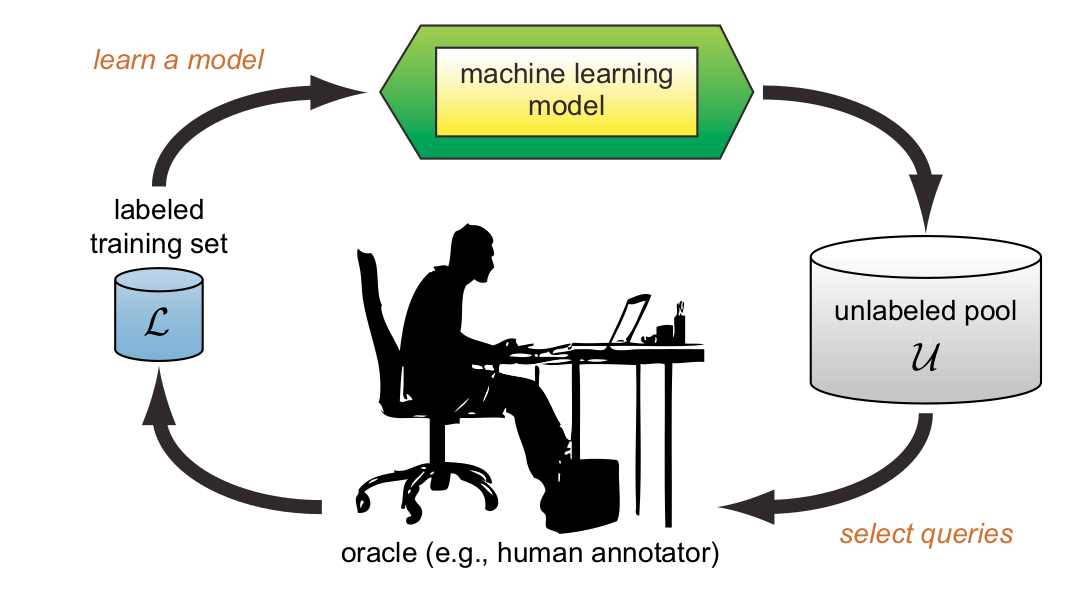
\includegraphics[scale=0.3]{images/active_learning.png}
    \end{figure}
\end{frame}

\begin{frame}[fragile]{Active Learning}
    \begin{figure}[htp]
        \centering
        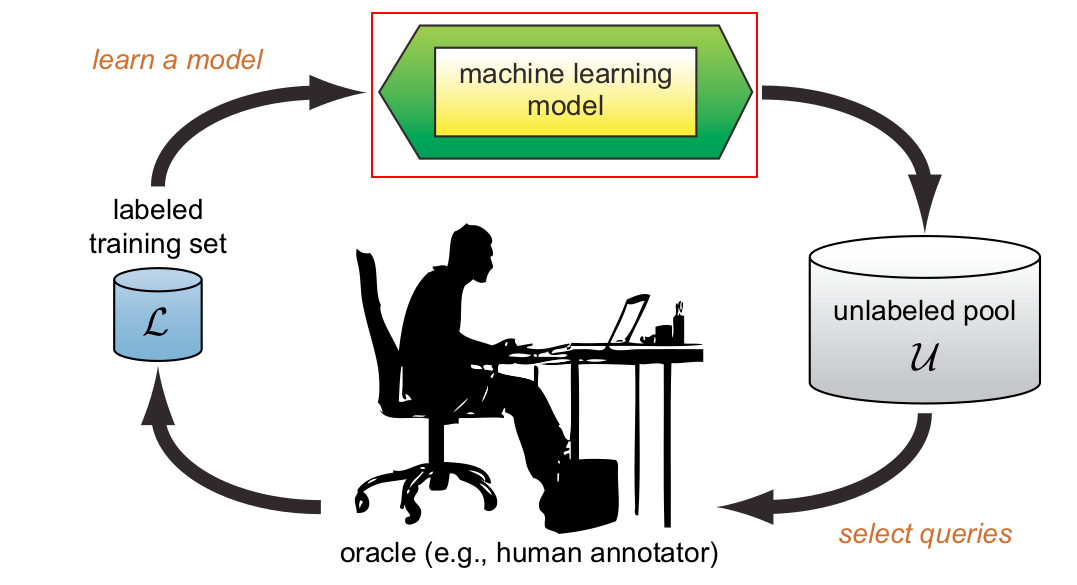
\includegraphics[scale=0.3]{images/active_learning_ml_model.png}
    \end{figure}
\end{frame}

\begin{frame}[fragile]{Active Learning}
    \begin{figure}[htp]
        \centering
        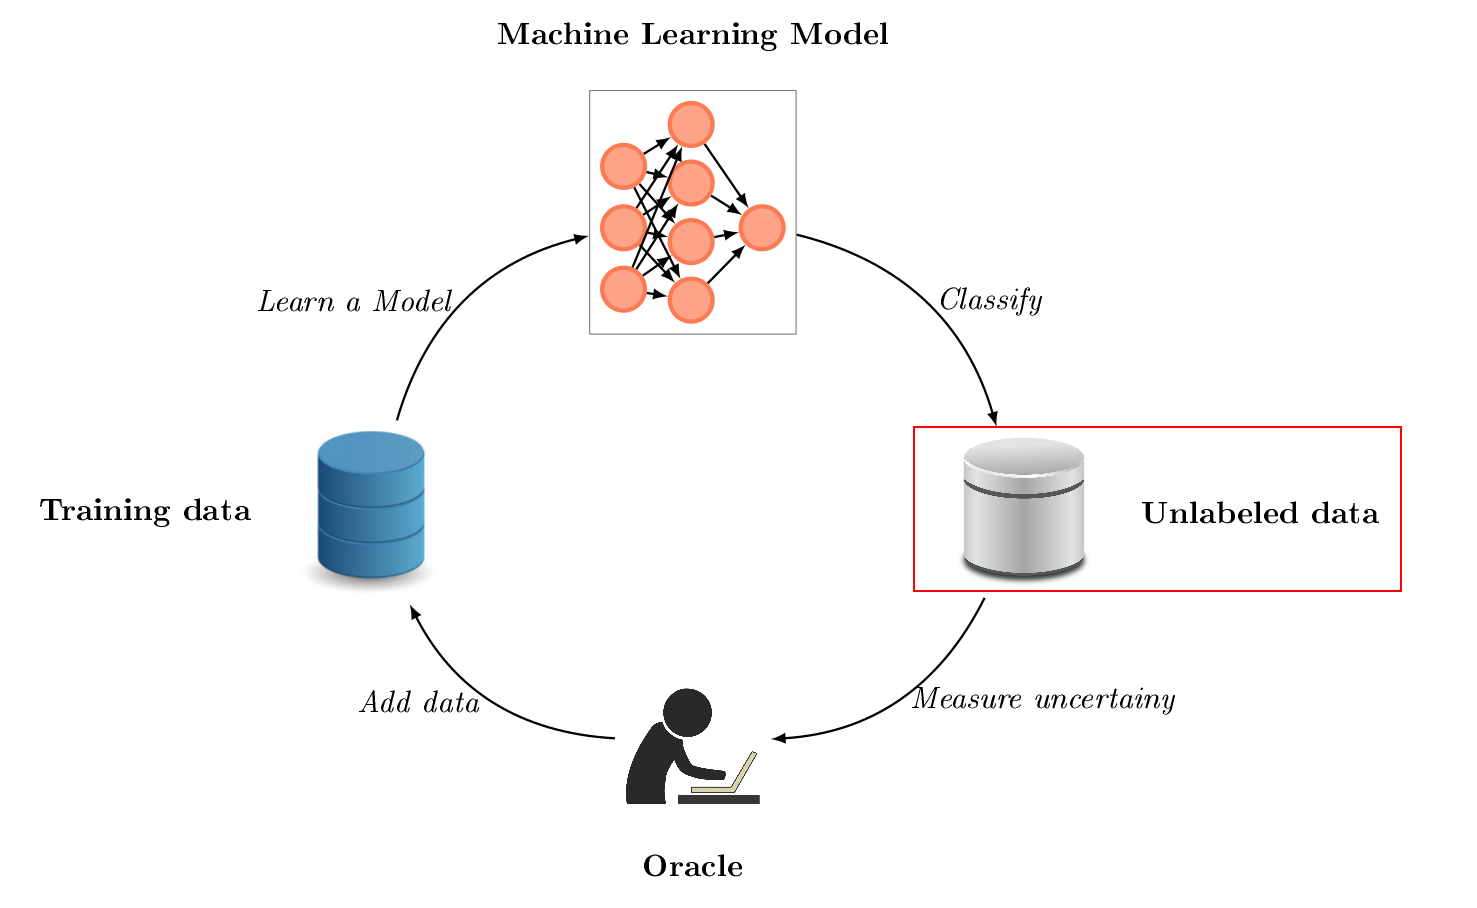
\includegraphics[scale=0.3]{images/active_learning_unlabeled.png}
    \end{figure}
\end{frame}

\begin{frame}[fragile]{Active Learning}
    \begin{figure}[htp]
        \centering
        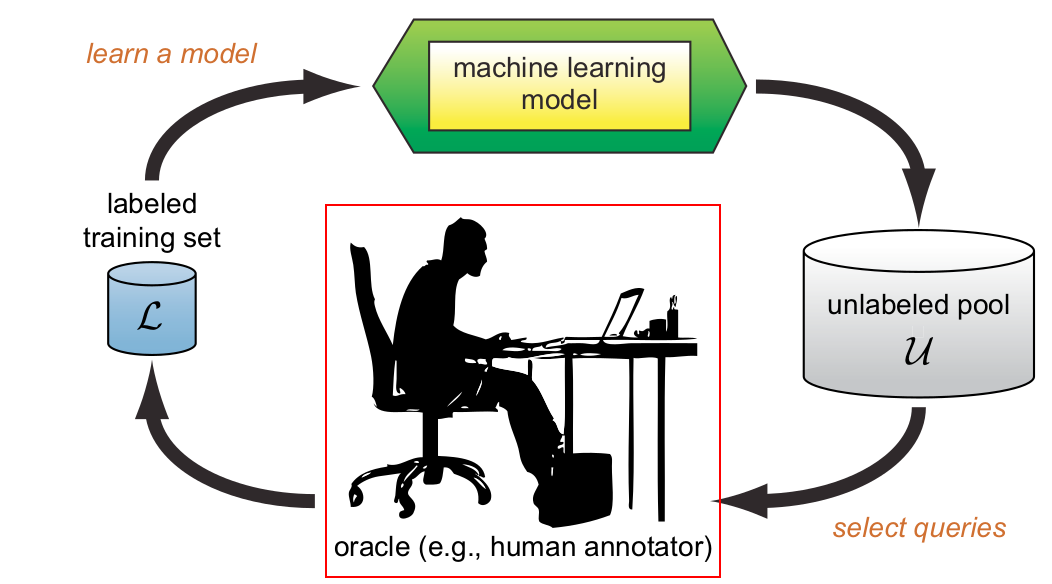
\includegraphics[scale=0.3]{images/active_learning_oracle.png}
    \end{figure}
\end{frame}

\begin{frame}[fragile]{Active Learning}
    \begin{figure}[htp]
        \centering
        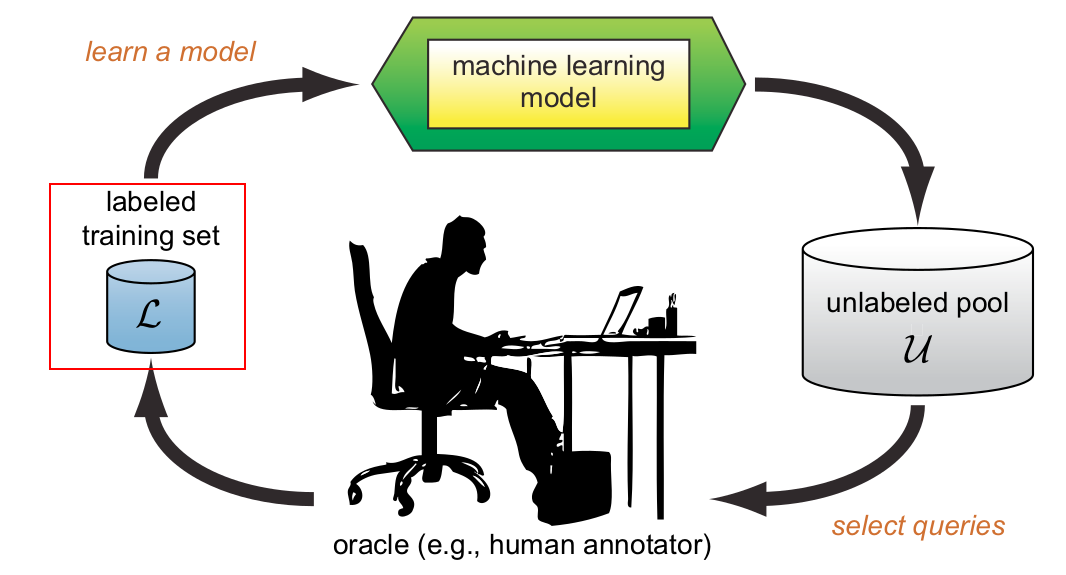
\includegraphics[scale=0.3]{images/active_learning_labeled.png}
    \end{figure}
\end{frame}

\begin{frame}[fragile]{Active Learning - CEAL}
    %\usetikzlibrary{fit}

\begin{figure}[ht!]
\centering

\scalebox{0.7}{
\begin{tikzpicture}[auto]

% operations =============================
\node[op] (x2) {};
\node[op, above=5pt of x2] (x1) {};
\node[op, below=5pt of x2] (x3) {};
\node[op, above right=4pt and 12pt of x2] (h2) {};
\node[op, above=4pt of h2] (h1) {};
\node[op, below=4pt of h2] (h3) {};
\node[op, below=4pt of h3] (h4) {};
\node[op, right=32pt of x2] (o) {};

% edges
\path[tedge] (x1) edge node[pos=0.25, above=1.8pt] {} (h1);
\path[tedge] (x1) edge node[above=1.2pt] {} (h2);
\path[tedge] (x1) edge node[above=1.8pt] {} (h3);
\path[tedge] (x1) edge node[above=1.8pt] {} (h4);

\path[tedge] (x2) edge node[above=1.8pt] {} (h1);
\path[tedge] (x2) edge node[above=1.8pt] {} (h2);
\path[tedge] (x2) edge node[above=1.8pt] {} (h3);
\path[tedge] (x2) edge node[above=1.8pt] {} (h4);

\path[tedge] (x3) edge node[above=1.8pt] {} (h1);
\path[tedge] (x3) edge node[above=1.8pt] {} (h2);
\path[tedge] (x3) edge node[above=1.8pt] {} (h3);
\path[tedge] (x3) edge node[above=1.0pt] {} (h4);

\path[tedge] (h1) edge node[pos=0.25, above=1.8pt, right=0.1cm] {} (o);
\path[tedge] (h2) edge node[above=1.8pt] {} (o);
\path[tedge] (h3) edge node[above=1.8pt] {} (o);
\path[tedge] (h4) edge node[above=1.8pt] {} (o);

\node [draw=black!50, fit={(x1) (x2) (x3) (h1) (h2) (h3) (h4) (o)}] (nn) {};

\node[below left=30pt and 50pt of nn] (tdata)
    {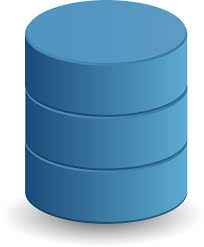
\includegraphics[width=.1\textwidth]{images/training_dataset}};

\node[right=175pt of tdata] (udata)
    {
\includegraphics[width=.1\textwidth]{images/unlabeled_dataset}};

\node[below=120pt of nn] (oracle)
    {
\includegraphics[width=.1\textwidth]{images/oracle}};

\node[textonly, left=10pt of tdata] (tdatalabel) {\textbf{Training data}};
\node[textonly, right=10pt of udata] (udatalabel) {\textbf{Unlabeled data}};
\node[textonly, above=10pt of nn] (nnlabel) {\textbf{Machine Learning Model}};
\node[textonly, below=10pt of oracle] (oraclelabel) {\textbf{Oracle}};

\path[tedge] (tdata) edge[bend left, left] node {\textit{Learn a Model}} (nn);
\path[tedge] (nn) edge[bend left, right] node {\textit{Classify}} (udata);
\path[tedge] (nn) edge[bend left, right] node {\textit{Remove CEAL examples}} (tdata);
\path[tedge] (udata) edge[bend left, right] node {\textit{Measure uncertainy}} (oracle);
\path[tedge] (oracle) edge[bend left, left] node {\textit{Add data}} (tdata);
\path[tedge] (udata) edge node[pos=0.5, below=1.8pt] {Add CEAL Examples} (tdata);


\end{tikzpicture}
} % scalebox
\end{figure}

\end{frame}

\begin{frame}[fragile]{Active Learning}
    \begin{figure}[htp]
        \centering
        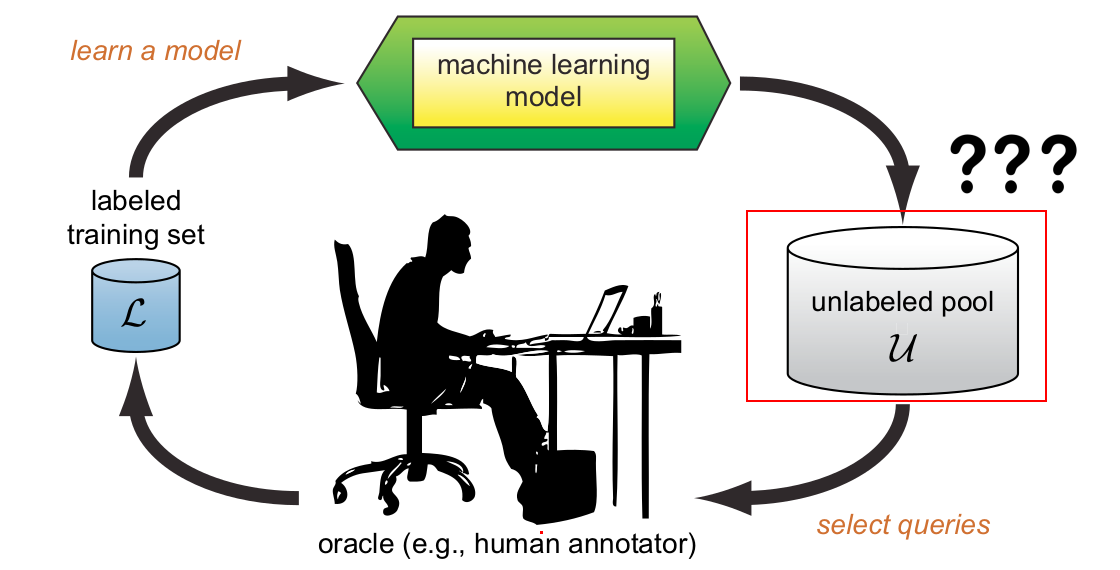
\includegraphics[scale=0.3]{images/active_learning_uncertainty.png}
    \end{figure}
\end{frame}

\begin{frame}[fragile]{Uncertainty measurement}
\begin{itemize}
\item To select informative samples, it is necessary to measure the
    \alert{uncertainty} of the model prediction.
\end{itemize}
\end{frame}

\begin{frame}[fragile]{Neural Network}
    \begin{figure}[ht!]
\centering

\scalebox{1.0}{
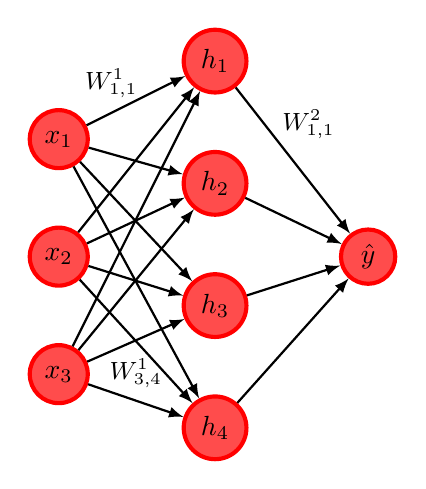
\begin{tikzpicture}[auto]

% operations =============================
\node[op] (x2) {$x_2$};
\node[op, above=20pt of x2] (x1) {$x_1$};
\node[op, below=20pt of x2] (x3) {$x_3$};
\node[op, above right=10pt and 40pt of x2] (h2) {$h_2$};
\node[op, above=20pt of h2] (h1) {$h_1$};
\node[op, below=20pt of h2] (h3) {$h_3$};
\node[op, below=20pt of h3] (h4) {$h_4$};
\node[op, right=90pt of x2] (y) {$\hat{y}$};

% edges
\path[tedge] (x1) edge node[pos=0.25, above=1.8pt] {\alert{\small $\vect{W}_{1,1}^{1}$}} (h1);
\path[tedge] (x1) edge node[above=1.2pt] {} (h2);
\path[tedge] (x1) edge node[above=1.8pt] {} (h3);
\path[tedge] (x1) edge node[above=1.8pt] {} (h4);

\path[tedge] (x2) edge node[above=1.8pt] {} (h1);
\path[tedge] (x2) edge node[above=1.8pt] {} (h2);
\path[tedge] (x2) edge node[above=1.8pt] {} (h3);
\path[tedge] (x2) edge node[above=1.8pt] {} (h4);

\path[tedge] (x3) edge node[above=1.8pt] {} (h1);
\path[tedge] (x3) edge node[above=1.8pt] {} (h2);
\path[tedge] (x3) edge node[above=1.8pt] {} (h3);
\path[tedge] (x3) edge node[above=1.0pt] {\small $\vect{W}_{3,4}^{1}$} (h4);

\path[tedge] (h1) edge node[pos=0.25, above=1.8pt, right=0.1cm] {\small $\vect{W}_{1,1}^{2}$} (y);
\path[tedge] (h2) edge node[above=1.8pt] {} (y);
\path[tedge] (h3) edge node[above=1.8pt] {} (y);
\path[tedge] (h4) edge node[above=1.8pt] {} (y);

% info edges


\end{tikzpicture}
} % scalebox
\end{figure}

\end{frame}

\begin{frame}[fragile]{Bayesian Neural Network - prediction}
    \begin{figure}[htp]
        \centering
        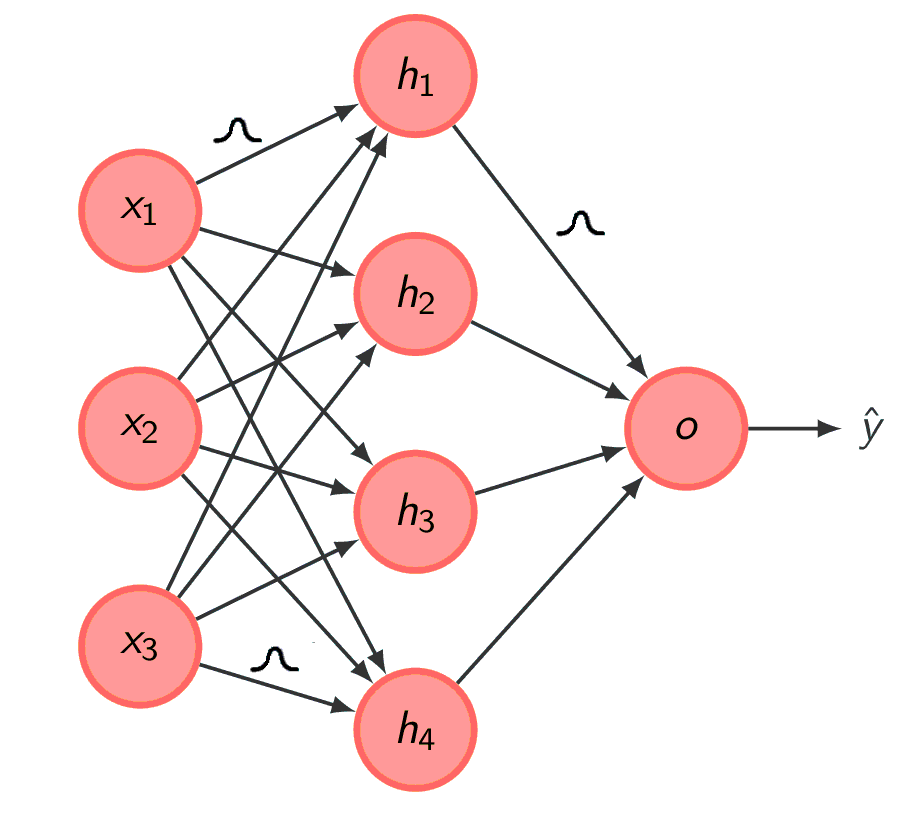
\includegraphics[scale=0.3]{images/bayesian_neural_network.png}
    \end{figure}
\end{frame}

\begin{frame}[fragile]{Bayesian Neural Network - prediction}
    \begin{figure}[ht!]
\centering

\scalebox{1.2}{
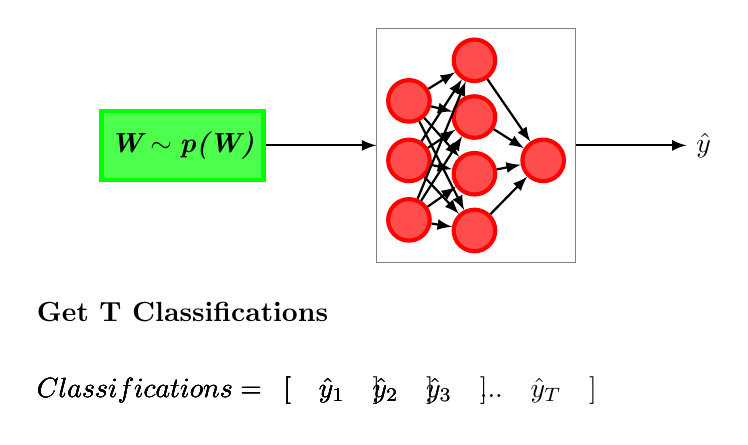
\begin{tikzpicture}[auto]

% operations =============================

\visible<2->{
\node[op] (x2) {};
\node[op, above=5pt of x2] (x1) {};
\node[op, below=5pt of x2] (x3) {};
\node[op, above right=4pt and 12pt of x2] (h2) {};
\node[op, above=4pt of h2] (h1) {};
\node[op, below=4pt of h2] (h3) {};
\node[op, below=4pt of h3] (h4) {};
\node[op, right=32pt of x2] (o) {};

% edges
\path[tedge] (x1) edge node[pos=0.25, above=1.8pt] {} (h1);
\path[tedge] (x1) edge node[above=1.2pt] {} (h2);
\path[tedge] (x1) edge node[above=1.8pt] {} (h3);
\path[tedge] (x1) edge node[above=1.8pt] {} (h4);

\path[tedge] (x2) edge node[above=1.8pt] {} (h1);
\path[tedge] (x2) edge node[above=1.8pt] {} (h2);
\path[tedge] (x2) edge node[above=1.8pt] {} (h3);
\path[tedge] (x2) edge node[above=1.8pt] {} (h4);

\path[tedge] (x3) edge node[above=1.8pt] {} (h1);
\path[tedge] (x3) edge node[above=1.8pt] {} (h2);
\path[tedge] (x3) edge node[above=1.8pt] {} (h3);
\path[tedge] (x3) edge node[above=1.0pt] {} (h4);

\path[tedge] (h1) edge node[pos=0.25, above=1.8pt, right=0.1cm] {} (o);
\path[tedge] (h2) edge node[above=1.8pt] {} (o);
\path[tedge] (h3) edge node[above=1.8pt] {} (o);
\path[tedge] (h4) edge node[above=1.8pt] {} (o);

\node [draw=black!50, fit={(x1) (x2) (x3) (h1) (h2) (h3) (h4) (o)}] (nn) {};
% edges
}

\node[rectangle, left=40pt of nn] (w) {$\textit{W} \sim \textit{p(W)}$};

\visible<2->{
  \path[tedge] (w) edge node[above=1.8pt] {} (nn);
}

\visible<3->{
\node[textonly, right=40pt of nn] (y) {$\hat{y}$};
\path[tedge] (nn) edge node[above=1.8pt] {} (y);
}

\visible<4->{
\node[textonly, below=40pt of w] (t_text) {Get T Classifications};
}

\visible<5>{
\node[textonly, right, below=of t_text.west,anchor=west] (a1) {$
  Classifications = \begin{array}{ccc}[& \hat{y}_{1} & ]\end{array}
$};
}

\visible<6>{
\node[textonly, below=of t_text.west,anchor=west] (a1) {$
  Classifications = \begin{array}{cccc}[& \hat{y}_{1} & \hat{y}_{2} & ]\end{array}
$};
}

\visible<7>{
\node[textonly, below=of t_text.west,anchor=west] (a1) {$
  Classifications = \begin{array}{ccccc}[& \hat{y}_{1} & \hat{y}_{2} &
  \hat{y}_{3} & ]\end{array}
$};
}

\visible<8>{
\node[textonly, below=of t_text.west,anchor=west] (a1) {$
Classifications = \begin{array}{ccccccc}[& \hat{y}_{1} & \hat{y}_{2} &
\hat{y}_{3} & ... & \hat{y}_{T} & ]\end{array}
$};
}

\end{tikzpicture}
} % scalebox
\end{figure}

\end{frame}

\begin{frame}[fragile]{Bayesian Neural Network - prediction}
\begin{itemize}
\item Training Bayesian networks is a costly process
\vspace{0.5cm}
\item Use techniques such as Variational Inference
\end{itemize}
\end{frame}

\begin{frame}[fragile]{Bayesian Neural Network}
\begin{itemize}
\item What if we could extract uncertainty measurements from current Deep
    Learning models if they use stochastic regularization techniques such as
    \alert{Dropout} ?
\vspace{0.5cm}
\item Uncertainty in Deep Learning (Yarin Gal, 2017)
\end{itemize}
\end{frame}

\section{Dropout}

\begin{frame}[fragile]{Dropout}
\begin{itemize}
\item During training some weights are dropped from the network
\end{itemize}
\end{frame}

\begin{frame}[fragile]{Dropout}
    \begin{figure}[ht!]
\centering

\scalebox{1.0}{
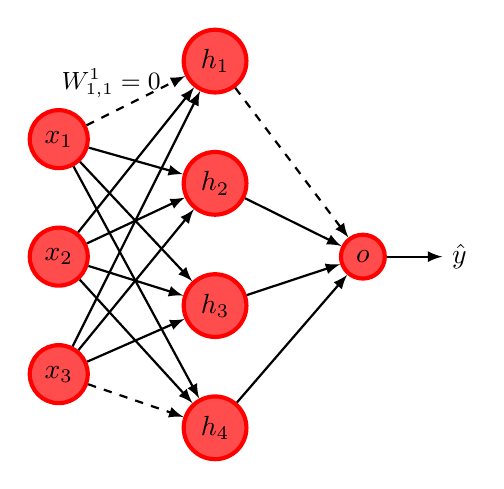
\begin{tikzpicture}[auto]

% operations =============================
\node[op] (x2) {$x_2$};
\node[op, above=20pt of x2] (x1) {$x_1$};
\node[op, below=20pt of x2] (x3) {$x_3$};
\node[op, above right=10pt and 40pt of x2] (h2) {$h_2$};
\node[op, above=20pt of h2] (h1) {$h_1$};
\node[op, below=20pt of h2] (h3) {$h_3$};
\node[op, below=20pt of h3] (h4) {$h_4$};
\node[op, right=90pt of x2] (o) {$o$};
\node[textonly, right=20pt of o] (y) {$\hat{y}$};

% edges
\path[tedge_dashed] (x1) edge node[pos=0.25, above=1.8pt, dashed] {
  \small $\vect{W}_{1,1}^{1} = 0$} (h1);
\path[tedge] (x1) edge node[above=1.2pt] {} (h2);
\path[tedge] (x1) edge node[above=1.8pt] {} (h3);
\path[tedge] (x1) edge node[above=1.8pt] {} (h4);

\path[tedge] (x2) edge node[above=1.8pt] {} (h1);
\path[tedge] (x2) edge node[above=1.8pt] {} (h2);
\path[tedge] (x2) edge node[above=1.8pt] {} (h3);
\path[tedge] (x2) edge node[above=1.8pt] {} (h4);

\path[tedge] (x3) edge node[above=1.8pt] {} (h1);
\path[tedge] (x3) edge node[above=1.8pt] {} (h2);
\path[tedge] (x3) edge node[above=1.8pt] {} (h3);
\path[tedge_dashed] (x3) edge node[above=1.0pt] {} (h4);

\path[tedge_dashed] (h1) edge node[pos=0.25, above=1.8pt, right=0.1cm] {} (o);
\path[tedge] (h2) edge node[above=1.8pt] {} (o);
\path[tedge] (h3) edge node[above=1.8pt] {} (o);
\path[tedge] (h4) edge node[above=1.8pt] {} (o);

\path[tedge] (o) edge node[above=1.8pt] {} (y);

% info edges


\end{tikzpicture}
} % scalebox
\end{figure}

\end{frame}

\begin{frame}[fragile]{Dropout}
    \begin{figure}[ht!]
\centering

\scalebox{1.0}{
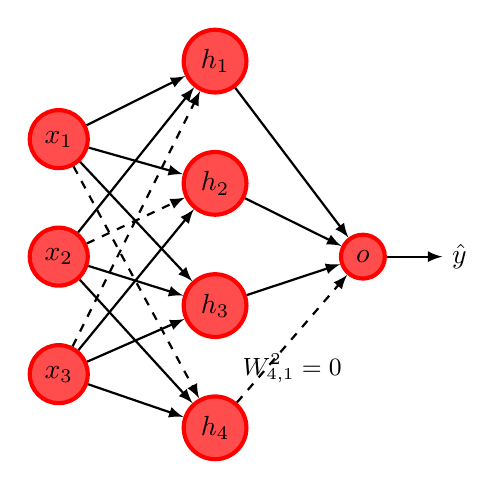
\begin{tikzpicture}[auto]

% operations =============================
\node[op] (x2) {$x_2$};
\node[op, above=20pt of x2] (x1) {$x_1$};
\node[op, below=20pt of x2] (x3) {$x_3$};
\node[op, above right=10pt and 40pt of x2] (h2) {$h_2$};
\node[op, above=20pt of h2] (h1) {$h_1$};
\node[op, below=20pt of h2] (h3) {$h_3$};
\node[op, below=20pt of h3] (h4) {$h_4$};
\node[op, right=90pt of x2] (o) {$o$};
\node[textonly, right=20pt of o] (y) {$\hat{y}$};

% edges
\path[tedge] (x1) edge node[pos=0.25, above=1.8pt] {} (h1);
\path[tedge] (x1) edge node[above=1.2pt] {} (h2);
\path[tedge] (x1) edge node[above=1.8pt] {} (h3);
\path[tedge_dashed] (x1) edge node[above=1.8pt] {} (h4);

\path[tedge] (x2) edge node[above=1.8pt] {} (h1);
\path[tedge_dashed] (x2) edge node[above=1.8pt] {} (h2);
\path[tedge] (x2) edge node[above=1.8pt] {} (h3);
\path[tedge] (x2) edge node[above=1.8pt] {} (h4);

\path[tedge_dashed] (x3) edge node[above=1.8pt] {} (h1);
\path[tedge] (x3) edge node[above=1.8pt] {} (h2);
\path[tedge] (x3) edge node[above=1.8pt] {} (h3);
\path[tedge] (x3) edge node[above=1.0pt] {} (h4);

\path[tedge] (h1) edge node[pos=0.25, above=1.8pt, right=0.1cm] {} (o);
\path[tedge] (h2) edge node[above=1.8pt] {} (o);
\path[tedge] (h3) edge node[above=1.8pt] {} (o);
\path[tedge_dashed] (h4) edge node[below=1.8pt] {\small $\vect{W}_{4,1}^{2} = 0$}(o);

\path[tedge] (o) edge node[above=1.8pt] {} (y);

% info edges


\end{tikzpicture}
} % scalebox
\end{figure}

\end{frame}

\begin{frame}[fragile]{Dropout}
\begin{itemize}
    \item The optimization function of Neural Networks using \alert{Dropout} is practically the same
        as the optimization function of a Network trained with Variational
        Inference.
    \vspace{0.5cm}
    \item Therefore it is possible to extract uncertainty measures from these
        networks, a technique called \alert{Monte Carlo Dropout}.
\end{itemize}
\end{frame}

\begin{frame}[fragile]{Monte Carlo Dropout - Prediction}
    \begin{figure}[ht!]
\centering

\scalebox{1.0}{
\begin{tikzpicture}[auto]

% operations =============================

\visible<3->{
\node[op] (x2) {};
\node[op, above=5pt of x2] (x1) {};
\node[op, below=5pt of x2] (x3) {};
\node[op, above right=4pt and 16pt of x2] (h2) {};
\node[op, above=4pt of h2] (h1) {};
\node[op, below=4pt of h2] (h3) {};
\node[op, below=4pt of h3] (h4) {};
\node[op, right=32pt of x2] (o) {};

% edges
\path[tedge] (x1) edge node[pos=0.25, above=1.8pt] {} (h1);
\path[tedge] (x1) edge node[above=1.2pt] {} (h2);
\path[tedge] (x1) edge node[above=1.8pt] {} (h3);
\path[tedge] (x1) edge node[above=1.8pt] {} (h4);

\path[tedge] (x2) edge node[above=1.8pt] {} (h1);
\path[tedge_dashed] (x2) edge node[above=1.8pt] {} (h2);
\path[tedge] (x2) edge node[above=1.8pt] {} (h3);
\path[tedge] (x2) edge node[above=1.8pt] {} (h4);

\path[tedge] (x3) edge node[above=1.8pt] {} (h1);
\path[tedge] (x3) edge node[above=1.8pt] {} (h2);
\path[tedge_dashed] (x3) edge node[above=1.8pt] {} (h3);
\path[tedge] (x3) edge node[above=1.0pt] {} (h4);

\path[tedge_dashed] (h1) edge node[pos=0.25, above=1.8pt, right=0.1cm] {} (o);
\path[tedge] (h2) edge node[above=1.8pt] {} (o);
\path[tedge] (h3) edge node[above=1.8pt] {} (o);
\path[tedge] (h4) edge node[above=1.8pt] {} (o);

\node [draw=black!50, fit={(x1) (x2) (x3) (h1) (h2) (h3) (h4) (o)}] (nn) {};

% edges
\path[tedge] (w) edge node[above=1.8pt] {} (nn);
}

\node[rectangle, left=40pt of nn] (w) {\small$\textit{E} \sim \textit{Bernoulli}$};

\visible<2->{
\node[textonly, above=20pt of w] (e) {\small$
   Dropout = \begin{array}{cccccc}[& 0 & 1 & ... & 0 & ]\end{array} $};
\path[tedge] (w) edge node[above=1.8pt] {} (e);
}

\visible<4->{
\node[textonly, right=40pt of nn] (y) {$\hat{y}$};
\path[tedge] (nn) edge node[above=1.8pt] {} (y);
}

\visible<5->{
\node[textonly, below=40pt of w] (t_text) {Get T Classifications};
}

\visible<6>{
\node[textonly, right, below=of t_text.west,anchor=west] (a1) {$
  Classifications = \begin{array}{ccc}[& \hat{y}_{1} & ]\end{array}
$};
}

\visible<7>{
\node[textonly, below=of t_text.west,anchor=west] (a1) {$
  Classifications = \begin{array}{cccc}[& \hat{y}_{1} & \hat{y}_{2} & ]\end{array}
$};
}

\visible<8>{
\node[textonly, below=of t_text.west,anchor=west] (a1) {$
  Classifications = \begin{array}{ccccc}[& \hat{y}_{1} & \hat{y}_{2} &
  \hat{y}_{3} & ]\end{array}
$};
}

\visible<9>{
\node[textonly, below=of t_text.west,anchor=west] (a1) {$
Classifications = \begin{array}{ccccccc}[& \hat{y}_{1} & \hat{y}_{2} &
\hat{y}_{3} & ... & \hat{y}_{T} & ]\end{array}
$};
}

\end{tikzpicture}
} % scalebox
\end{figure}

\end{frame}

\begin{frame}[fragile]{Active Learning}
    \begin{figure}[htp]
        \centering
        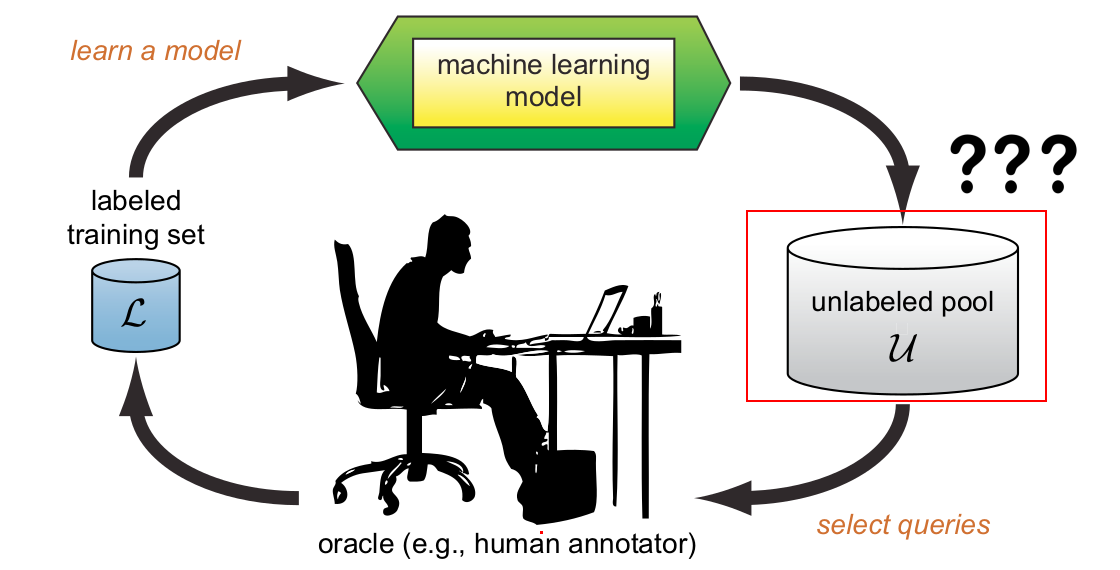
\includegraphics[scale=0.3]{images/active_learning_uncertainty.png}
    \end{figure}
\end{frame}

\begin{frame}[fragile]{Active Learning}
    \begin{figure}[htp]
        \centering
        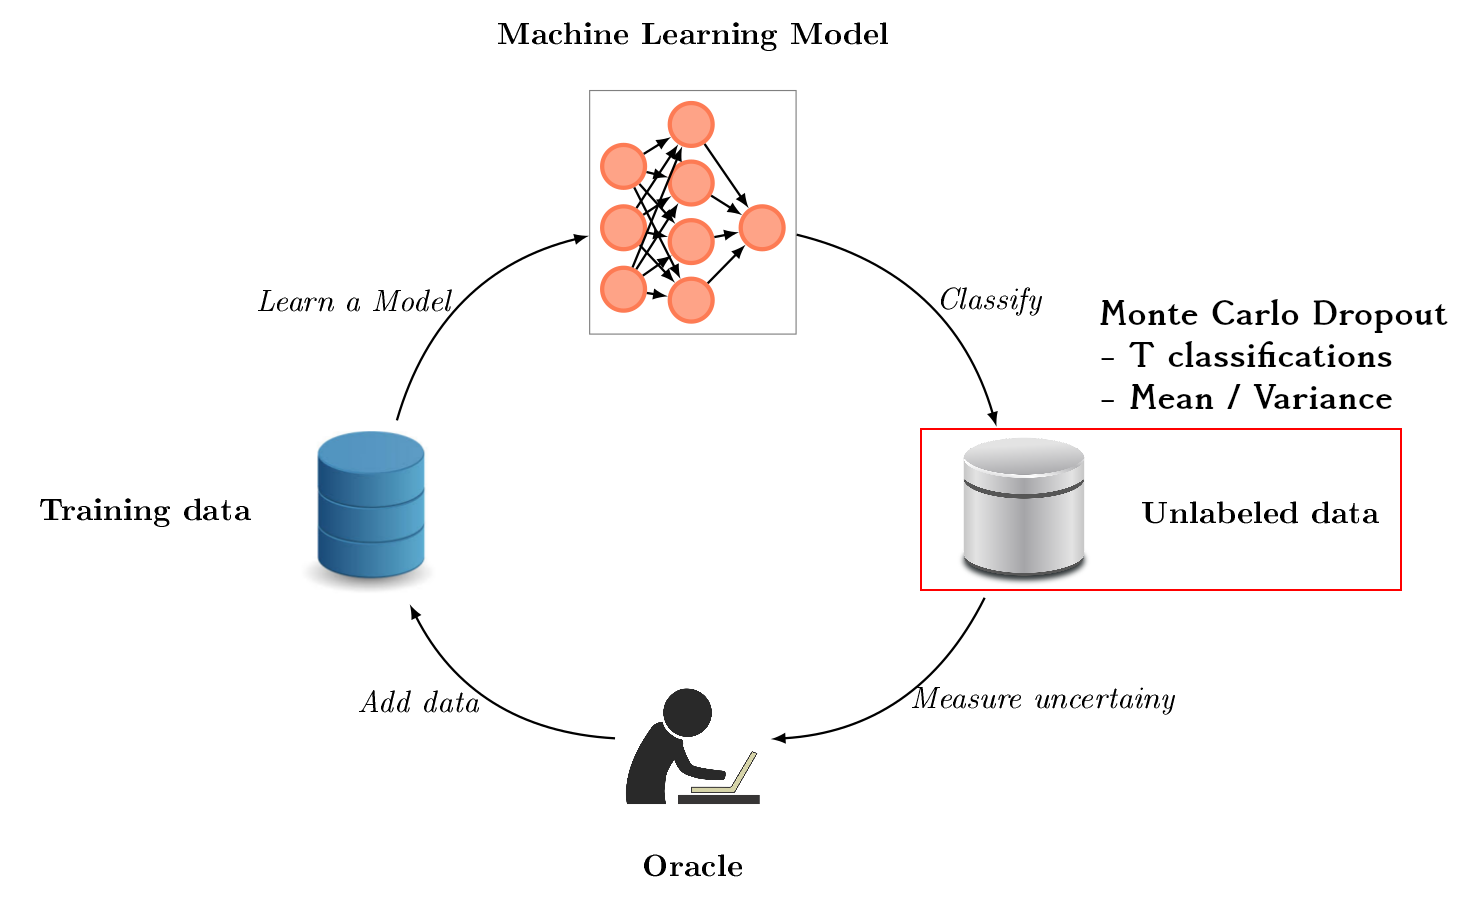
\includegraphics[scale=0.3]{images/active_learning_uncertainty_dropout.png}
    \end{figure}
\end{frame}

\section{Experimental Design}

\begin{frame}[fragile]{Research Contributions}
\begin{itemize}
\item An intrinsic comparison of Monte Carlo Dropout with random sampling strategies for the
Active Learning framework for the task of sentiment analysis.
\item An intrinsic comparison of Monte Carlo Dropout with the softmax uncertainty measurement
for the Active Learning framework for the task of sentiment analysis
\item Practical considerations when applying Deep Learning with Active Learning
\end{itemize}
\end{frame}

\begin{frame}[fragile]{Research Questions}
\begin{itemize}
    \item \alert{Q1}: On the task of sentiment analysis, does modelling the uncertainty measurement of the
    model using the Monte Carlo Dropout technique help us achieve a better accuracy value in
    the Active Learning context ?
    \vspace{0.5cm}
    \item \alert{Q2}: Does Monte Carlo Dropout
    provides best uncertainty measurements then using the softmax output as a uncertainty measurement, the classical approach used in DL models ?
\end{itemize}
\end{frame}

\begin{frame}[fragile]{Active Learning}
    \begin{figure}[htp]
        \centering
        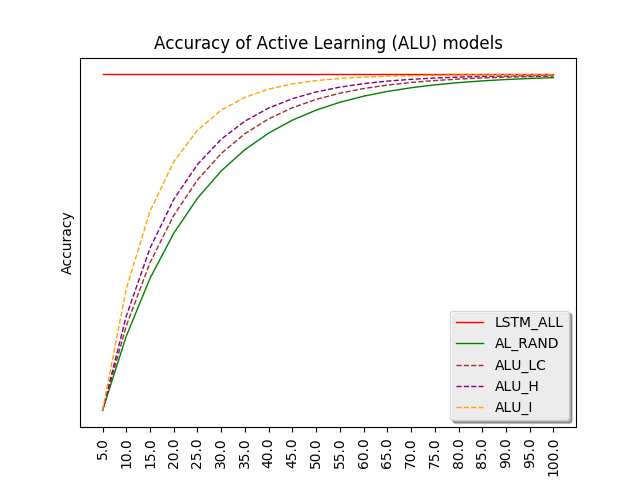
\includegraphics[scale=0.6]{images/active_learning_comp_graph.png}
    \end{figure}
\end{frame}

\begin{frame}[fragile]{Datasets}
\begin{itemize}
    \item Large Movie Review Dataset
    \begin{itemize}
    \item 25000 train reviews and 25000 test reviews
    \item Both train and test datasets have an equal number of positive and
        negative reviews
    \end{itemize}
    \vspace{0.5cm}
    \item Subjectivity Dataset
    \begin{itemize}
    \item 10000 movie reviews divided into subjective and objective text.
    \item Dataset perfectly balanced
    \item Reviews hava an average size of 20 words
    \end{itemize}
\end{itemize}
\end{frame}

\begin{frame}[fragile]{Network Archictecture}
    % RNN STATE CELL ====================================
\begin{figure}[ht!]
\centering
\hspace*{-1.0cm}
\scalebox{0.5}{

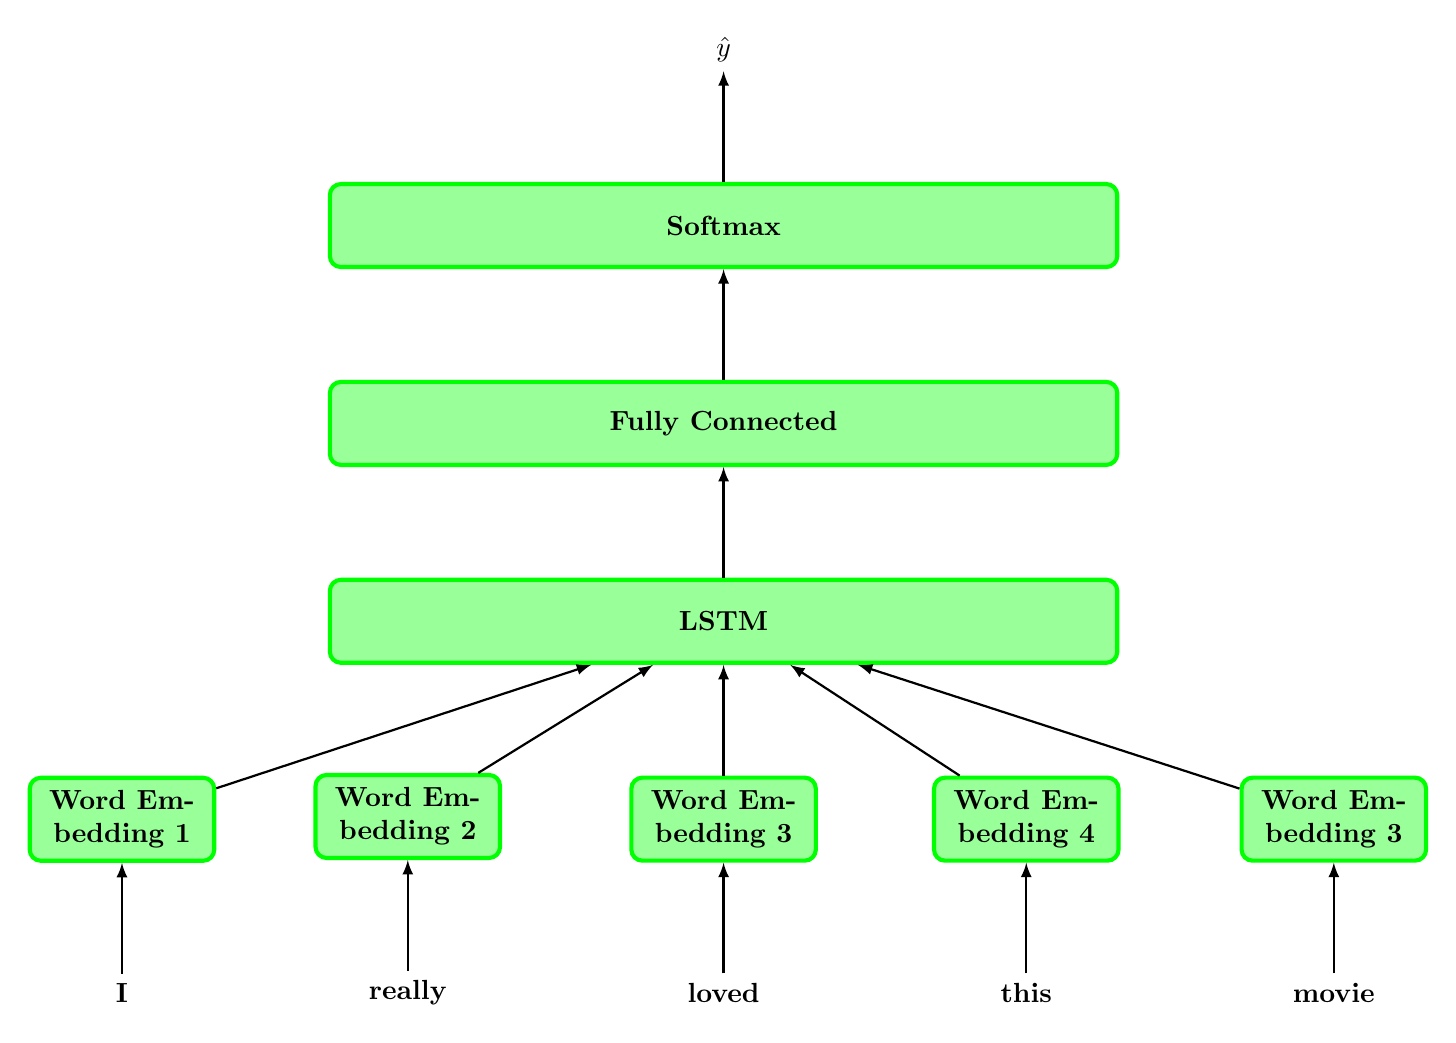
\begin{tikzpicture}[auto]

\node[textonly] (loved) {loved};
\node[textonly, left=80pt of loved] (really) {really};
\node[textonly, left=80pt of really] (I) {I};
\node[textonly, right=80pt of loved] (this) {this};
\node[textonly, right=80pt of this] (movie) {movie};

\node[block, fill=green!40, above=40pt of loved] (wordembedding3) {Word Embedding 3};
\node[block, fill=green!40, above=40pt of really] (wordembedding2) {Word Embedding 2};
\node[block, fill=green!40, above=40pt of I] (wordembedding1) {Word Embedding 1};
\node[block, fill=green!40, above=40pt of this] (wordembedding4) {Word Embedding 4};
\node[block, fill=green!40, above=40pt of movie] (wordembedding5) {Word Embedding 3};

\node[block, fill=green!40, minimum width=10cm, above=40pt of wordembedding3] (lstm) {LSTM};
\node[block, fill=green!40, minimum width=10cm, text width=9em, above=40pt of lstm] (fc) {Fully Connected};
\node[block, fill=green!40, minimum width=10cm, above=40pt of fc] (softmax) {Softmax};
\node[textonly, above=40pt of softmax] (prediction) {$\hat{y}$};

\path[tedge] (I) edge node[pos=0.25, above=1.8pt] {} (wordembedding1);
\path[tedge] (really) edge node[pos=0.25, above=1.8pt] {} (wordembedding2);
\path[tedge] (loved) edge node[above=1.2pt] {} (wordembedding3);
\path[tedge] (this) edge node[above=1.8pt] {} (wordembedding4);
\path[tedge] (movie) edge node[above=1.8pt] {} (wordembedding5);

\path[tedge] (wordembedding1) edge node[pos=0.25, above=1.8pt] {} (lstm);
\path[tedge] (wordembedding2) edge node[pos=0.25, above=1.8pt] {} (lstm);
\path[tedge] (wordembedding3) edge node[above=1.2pt] {} (lstm);
\path[tedge] (wordembedding4) edge node[above=1.8pt] {} (lstm);
\path[tedge] (wordembedding5) edge node[above=1.8pt] {} (lstm);

\path[tedge] (lstm) edge node[above=1.8pt] {} (fc);
\path[tedge] (fc) edge node[above=1.8pt] {} (softmax);
\path[tedge] (softmax) edge node[above=1.8pt] {} (prediction);

\end{tikzpicture}
}%\scalebox
\end{figure}

\end{frame}

\begin{frame}[fragile]{Experimental Design}
    \begin{figure}[ht!]
\centering

\scalebox{1.0}{
\begin{tikzpicture}[auto]

\visible<6->{
\node[rectangle, minimum size=15pt,
      draw=black!70,
      rounded corners=0.5pt,
      fill=red!70] (activemc) {ALU};
\path[tedge] (w) edge node[above=1.8pt] {} (activemc.west);
}

\visible<2->{
\node[rectangle, above=60pt of activemc.west, anchor=west,
    minimum size=15pt,
    draw=black!70,
    rounded corners=0.5pt,
    fill=red!70] (lstm) {LSTM model};
    \path[tedge] (w) edge node[above=1.8pt] {} (lstm.west);
}

\visible<4->{
\node[textonly, right=40pt of lstm] (lstmtrain) {Use whole training set};
\path[tedge] (lstm) edge node[above=1.8pt] {} (lstmtrain.west);
}

\visible<3->{
\node[textonly, above=10pt of lstmtrain.west, anchor=west] (lstmstandard) {Baseline model};
\path[tedge] (lstm) edge node[above=1.8pt] {} (lstmstandard.west);
}

\visible<5->{
\node[textonly, below=10pt of lstmtrain.west, anchor=west] (lstmhyper) {Hyperparameters tuning};
\path[tedge] (lstm) edge node[above=1.8pt] {} (lstmhyper.west);
}

\visible<9->{
    \node[textonly, right=80pt of activemc] (alulco) {Least Confident (LC)};
\path[tedge] (activemc) edge node[above=1.8pt] {} (alulco.west);
}

\visible<8->{
\node[textonly, above=10pt of alulco.west, anchor=west] (alumc) {MC Dropout};
\path[tedge] (activemc) edge node[above=1.8pt] {} (alumc.west);
}

\visible<7->{
\node[textonly, above=10pt of alumc.west, anchor=west] (aluname) {Active Learning + Uncertainty};
\path[tedge] (activemc) edge node[above=1.8pt] {} (aluname.west);
}

\visible<10->{
    \node[textonly, below=10pt of alulco.west, anchor=west] (aluh) {Entropy (H)};
\path[tedge] (activemc) edge node[above=1.8pt] {} (aluh.west);
}

\visible<11->{
\node[textonly, below=10pt of aluh.west, anchor=west] (alumi) {Mutual Information (I)};
\path[tedge] (activemc) edge node[above=1.8pt] {} (alumi.west);
}

\visible<12->{
\node[rectangle, below=60pt of activemc.west, anchor=west, minimum size=15pt,
      draw=black!70,
      rounded corners=0.5pt,
      fill=red!70] (actives) {ALS};
\path[tedge] (w) edge node[above=1.8pt] {} (actives.west);
}

\visible<15->{
\node[textonly, right=80pt of actives] (alslco) {Least Confident (LC)};
\path[tedge] (actives) edge node[above=1.8pt] {} (alslco.west);
}

\visible<14->{
\node[textonly, above=10pt of alslco.west, anchor=west] (alsmc) {Softmax};
\path[tedge] (actives) edge node[above=1.8pt] {} (alsmc.west);
}

\visible<13->{
\node[textonly, above=10pt of alsmc.west, anchor=west] (alsname) {Active Learning + Softmax};
\path[tedge] (actives) edge node[above=1.8pt] {} (alsname.west);
}

\visible<16->{
    \node[textonly, below=10pt of alslco.west, anchor=west] (alsh) {Entropy (H)};
\path[tedge] (actives) edge node[above=1.8pt] {} (alsh.west);
}

\visible<17->{
\node[textonly, below=10pt of alsh.west, anchor=west] (alsmi) {Mutual Information (I)};
\path[tedge] (actives) edge node[above=1.8pt] {} (alsmi.west);
}

\node[op, left=40pt of activemc, draw=black!50, fill=black] (w) {};

\end{tikzpicture}
} % scalebox
\end{figure}

\end{frame}

\begin{frame}[fragile]{Active Learning}
    \begin{figure}[htp]
        \centering
        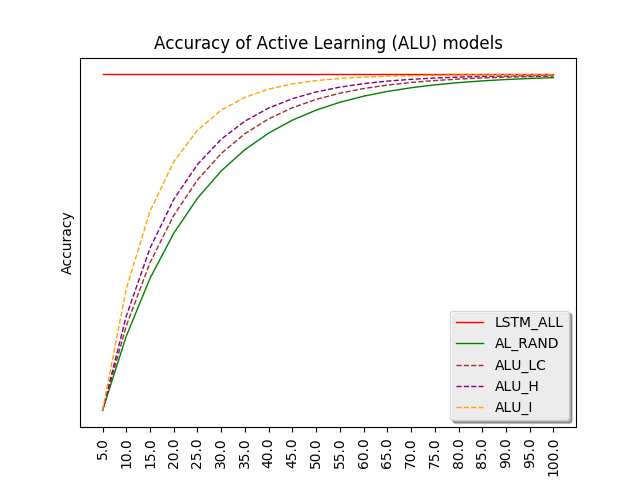
\includegraphics[scale=0.6]{images/active_learning_comp_graph.png}
    \end{figure}
\end{frame}

\begin{frame}[fragile]{Active Learning Experiments Parameters}
\begin{table}[]
\centering
\begin{tabular}{lll}
\toprule
Dataset & Labeled Group & Unlabeled Group\\
\midrule
\rowcolor{black!20}  Large Movie Review Dataset & 225 & 22275\\
Subjectivity Dataset & 10 & 8090\\
\bottomrule
\end{tabular}
\end{table}
\end{frame}


\begin{frame}[fragile]{Active Learning Experiments Parameters}
\begin{table}
\centering
\resizebox{\columnwidth}{!}{%
\begin{tabular}{ll}
\toprule
Parameter & Description\\
\midrule
\rowcolor{black!20} Unlabeled Data Queries (Q) & The number of example we will select from the unlabeled group\\
\rowcolor{black!20} & to be labeled by the oracle.\\
Number of epochs (EPO) & At each AL cycle, we will train our model for a given number of\\
& epochs. This variable defines this quantity.\\
\rowcolor{black!20} Dropout Values (DROP) & The dropout probability for the weights in our network.\\
Number of Active Learning Cycles (NC) & The number of AL cycles we have run for a given experiment.\\
\bottomrule
\end{tabular}%
}
\end{table}
\end{frame}


\section{Experiments Evaluation}

\begin{frame}[fragile]{First Iteration}
    \begin{itemize}
        \item Validate proposed model
        \item Find Hyperparameters
        \item Parameters
            \begin{itemize}
            \item \textbf{Q (Number of data added to training dataset)} = 50
            \item \textbf{EPO (Number of Epochs)} = 16
            \item \textbf{NC (Number of Active Learning Cycles)} = 50
            \end{itemize}
        \item Only one ALU model created (ALU\_I)
        \item Random and ALU\_I curve are almost identical
    \end{itemize}
\end{frame}

\begin{frame}[fragile]{Second Iteration}
\begin{itemize}
    \item Increase number of epochs in experiments
\end{itemize}
\end{frame}

\begin{frame}[fragile]{Second Iteration}
\begin{figure}[H]
    \centering
    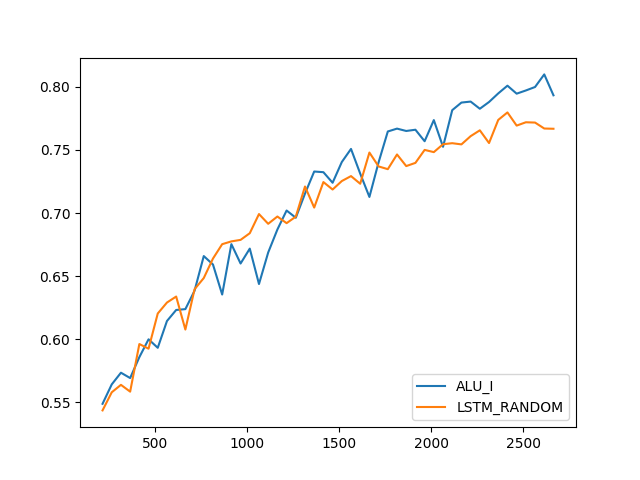
\includegraphics[width=0.7\textwidth]{images/acl_n200_comparison}
\end{figure}

\hspace{1.5cm} $\bullet$ \textbf{Q} = 50 \hspace{1cm} $\bullet$ \textbf{EPO} = 200 \hspace{1cm} $\bullet$ \textbf{NC} = 50
\end{frame}

\begin{frame}[fragile]{Third Iteration}
\begin{itemize}
    \item Decrease number of unlabeled examples added to training dataset
    \item Decrease number of epochs
    \item Increase Dropour values
\end{itemize}
\end{frame}

\begin{frame}[fragile]{Third Iteration}
\begin{figure}[H]
    \centering
    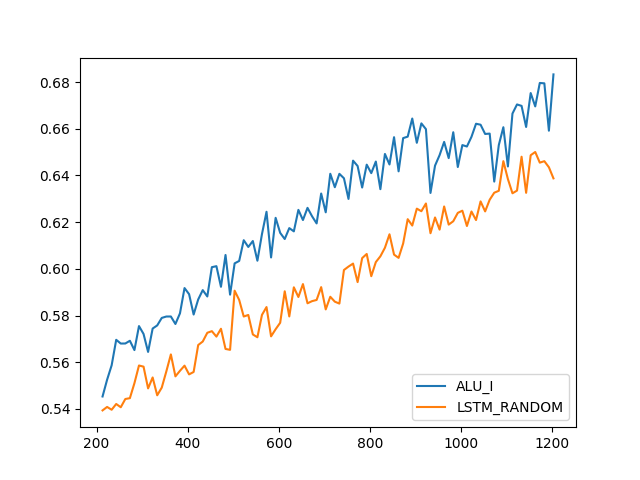
\includegraphics[width=0.7\textwidth]{images/acl_n150_q10_comparison}
\end{figure}

\hspace{0.5cm} $\bullet$ \textbf{Q} = 10 \hspace{0.5cm} $\bullet$ \textbf{EPO} = 150 \hspace{0.5cm}
$\bullet$ \textbf{NC} = 50 \hspace{0.5cm} \textbf{DROP} = 0.5
\end{frame}

\begin{frame}[fragile]{Third Iteration}
\begin{figure}[H]
    \centering
    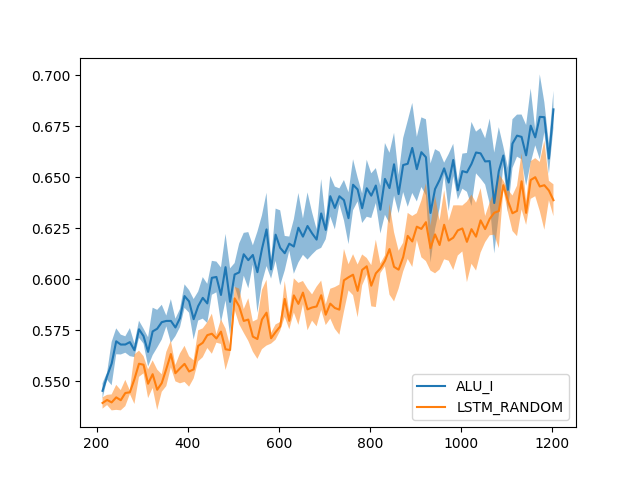
\includegraphics[width=0.7\textwidth]{images/acl_n150_q10_std_comparison}
\end{figure}

\hspace{0.5cm} $\bullet$ \textbf{Q} = 10 \hspace{0.5cm} $\bullet$ \textbf{EPO} = 150 \hspace{0.5cm}
$\bullet$ \textbf{NC} = 50 \hspace{0.5cm} \textbf{DROP} = 0.5
\end{frame}

\begin{frame}[fragile]{Fourth Iteration}
\begin{itemize}
    \item Compare all metrics
    \item Use CEAL approach
\end{itemize}
\end{frame}

\begin{frame}[fragile]{Fourth Iteration}
\begin{figure}[H]
    \centering
    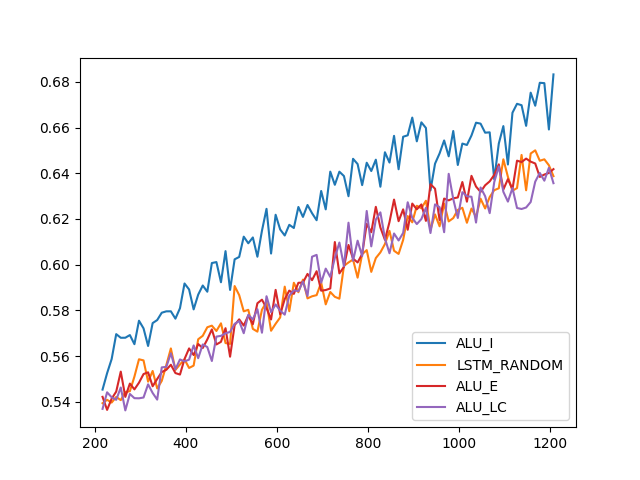
\includegraphics[width=0.7\textwidth]{images/acl_n150_q10_full_comparison}
\end{figure}

\hspace{0.5cm} $\bullet$ \textbf{Q} = 10 \hspace{0.5cm} $\bullet$ \textbf{EPO} = 150 \hspace{0.5cm} $\bullet$ \textbf{NC} = 100 \hspace{0.5cm} \textbf{DROP} = 0.5
\end{frame}

\begin{frame}[fragile]{Fourth Iteration}
    %\usetikzlibrary{fit}

\begin{figure}[ht!]
\centering

\scalebox{0.7}{
\begin{tikzpicture}[auto]

% operations =============================
\node[op] (x2) {};
\node[op, above=5pt of x2] (x1) {};
\node[op, below=5pt of x2] (x3) {};
\node[op, above right=4pt and 12pt of x2] (h2) {};
\node[op, above=4pt of h2] (h1) {};
\node[op, below=4pt of h2] (h3) {};
\node[op, below=4pt of h3] (h4) {};
\node[op, right=32pt of x2] (o) {};

% edges
\path[tedge] (x1) edge node[pos=0.25, above=1.8pt] {} (h1);
\path[tedge] (x1) edge node[above=1.2pt] {} (h2);
\path[tedge] (x1) edge node[above=1.8pt] {} (h3);
\path[tedge] (x1) edge node[above=1.8pt] {} (h4);

\path[tedge] (x2) edge node[above=1.8pt] {} (h1);
\path[tedge] (x2) edge node[above=1.8pt] {} (h2);
\path[tedge] (x2) edge node[above=1.8pt] {} (h3);
\path[tedge] (x2) edge node[above=1.8pt] {} (h4);

\path[tedge] (x3) edge node[above=1.8pt] {} (h1);
\path[tedge] (x3) edge node[above=1.8pt] {} (h2);
\path[tedge] (x3) edge node[above=1.8pt] {} (h3);
\path[tedge] (x3) edge node[above=1.0pt] {} (h4);

\path[tedge] (h1) edge node[pos=0.25, above=1.8pt, right=0.1cm] {} (o);
\path[tedge] (h2) edge node[above=1.8pt] {} (o);
\path[tedge] (h3) edge node[above=1.8pt] {} (o);
\path[tedge] (h4) edge node[above=1.8pt] {} (o);

\node [draw=black!50, fit={(x1) (x2) (x3) (h1) (h2) (h3) (h4) (o)}] (nn) {};

\node[below left=30pt and 50pt of nn] (tdata)
    {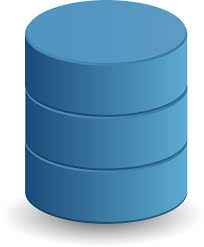
\includegraphics[width=.1\textwidth]{images/training_dataset}};

\node[right=175pt of tdata] (udata)
    {
\includegraphics[width=.1\textwidth]{images/unlabeled_dataset}};

\node[below=120pt of nn] (oracle)
    {
\includegraphics[width=.1\textwidth]{images/oracle}};

\node[textonly, left=10pt of tdata] (tdatalabel) {\textbf{Training data}};
\node[textonly, right=10pt of udata] (udatalabel) {\textbf{Unlabeled data}};
\node[textonly, above=10pt of nn] (nnlabel) {\textbf{Machine Learning Model}};
\node[textonly, below=10pt of oracle] (oraclelabel) {\textbf{Oracle}};

\path[tedge] (tdata) edge[bend left, left] node {\textit{Learn a Model}} (nn);
\path[tedge] (nn) edge[bend left, right] node {\textit{Classify}} (udata);
\path[tedge] (nn) edge[bend left, right] node {\textit{Remove CEAL examples}} (tdata);
\path[tedge] (udata) edge[bend left, right] node {\textit{Measure uncertainy}} (oracle);
\path[tedge] (oracle) edge[bend left, left] node {\textit{Add data}} (tdata);
\path[tedge] (udata) edge node[pos=0.5, below=1.8pt] {Add CEAL Examples} (tdata);


\end{tikzpicture}
} % scalebox
\end{figure}

\end{frame}

\begin{frame}[fragile]{Fourth Iteration}
\begin{figure}[H]
    \centering
    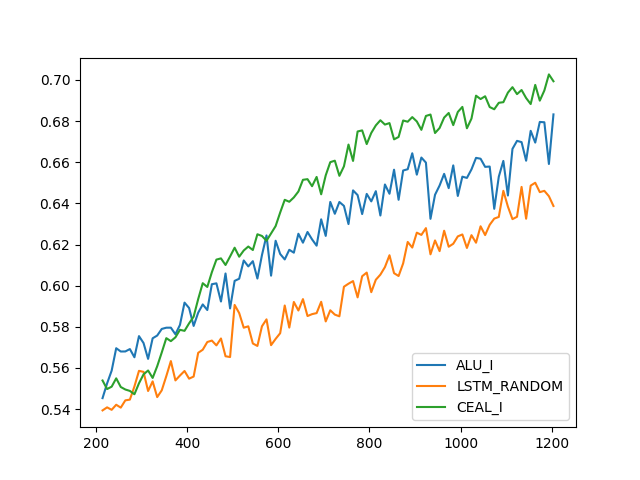
\includegraphics[width=0.7\textwidth]{images/acl_n150_q10_ceal_comparison}
\end{figure}

\end{frame}

\begin{frame}[fragile]{Fifth Iteration}
\begin{itemize}
    \item Compare softmax metric
\end{itemize}
\end{frame}

\begin{frame}[fragile]{Fifth Iteration}
\begin{figure}[H]
    \centering
    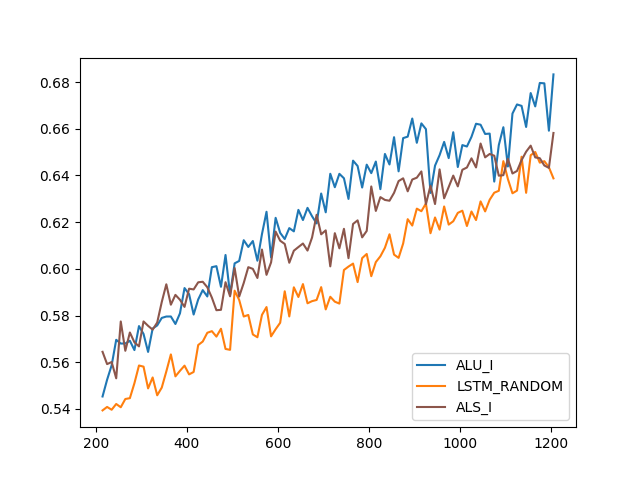
\includegraphics[width=0.7\textwidth]{images/acl_n150_q10_softmax_bald_comparison}
\end{figure}

\hspace{0.5cm} $\bullet$ \textbf{Q} = 10 \hspace{0.5cm} $\bullet$ \textbf{EPO} = 150 \hspace{0.5cm} $\bullet$ \textbf{NC} = 100 \hspace{0.5cm} \textbf{DROP} = 0.5
\end{frame}

\begin{frame}[fragile]{Sixth Iteration}
\begin{itemize}
    \item Use Subjectivity Dataset
    \item Compare all metrics
    \item Use CEAL approach
    \item Make softmax comparison
\end{itemize}
\end{frame}

\begin{frame}[fragile]{Sixth Iteration}
\begin{figure}[H]
    \centering
    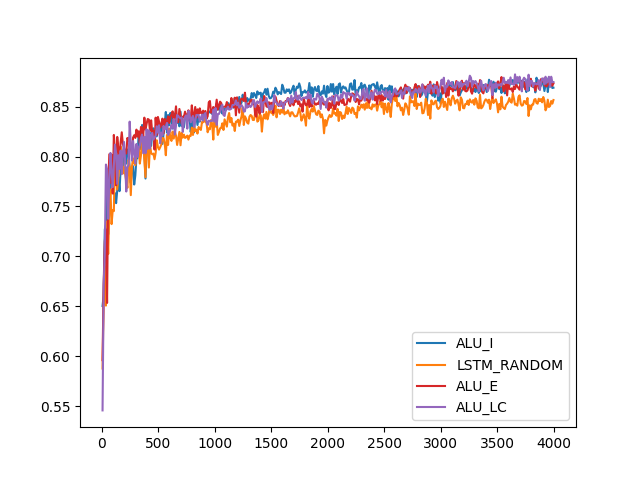
\includegraphics[width=0.7\textwidth]{images/subj_n150_q10_full_comparison}
\end{figure}

\hspace{0.5cm} $\bullet$ \textbf{Q} = 10 \hspace{0.5cm} $\bullet$ \textbf{EPO} = 150 \hspace{0.5cm} $\bullet$ \textbf{NC} = 400 \hspace{0.5cm} \textbf{DROP} = 0.5
\end{frame}

\begin{frame}[fragile]{Sixth Iteration}
\begin{figure}[H]
    \centering
    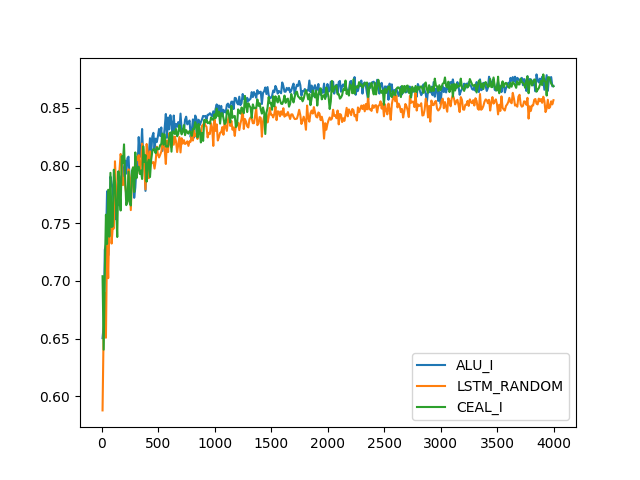
\includegraphics[width=0.7\textwidth]{images/subj_n150_q10_ceal_comparison}
\end{figure}

\hspace{0.5cm} $\bullet$ \textbf{Q} = 10 \hspace{0.5cm} $\bullet$ \textbf{EPO} = 150 \hspace{0.5cm} $\bullet$ \textbf{NC} = 400 \hspace{0.5cm} \textbf{DROP} = 0.5
\end{frame}

\begin{frame}[fragile]{Sixth Iteration}
\begin{figure}[H]
    \centering
    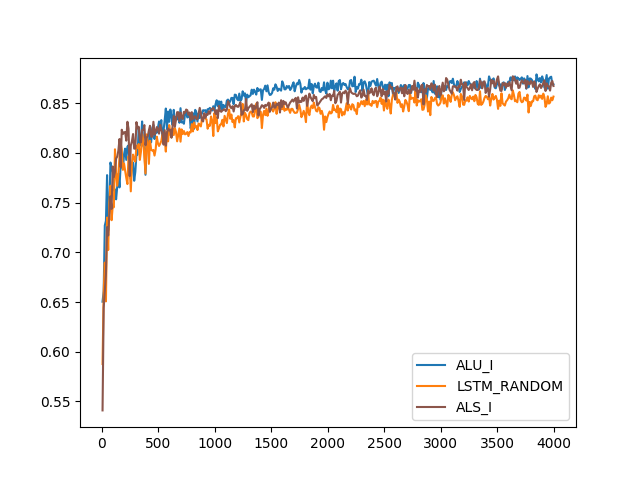
\includegraphics[width=0.7\textwidth]{images/subj_n150_q10_softmax_bald_comparison}
\end{figure}

\hspace{0.5cm} $\bullet$ \textbf{Q} = 10 \hspace{0.5cm} $\bullet$ \textbf{EPO} = 150 \hspace{0.5cm} $\bullet$ \textbf{NC} = 400 \hspace{0.5cm} \textbf{DROP} = 0.5
\end{frame}

\section{Conclusion}

\begin{frame}[fragile]{Conclusion}
\begin{itemize}
\item Measuring the uncertainty of sample using the Monte Carlo Dropout has created better
      accuracy curves than using both random and softmax.
\item We have positive results for both of our research questions
\item Not consistent result for both datasets
\end{itemize}
\end{frame}

\section{However}

\begin{frame}[fragile]{Active Learning Problems}
\begin{itemize}
\item LSTM is a bad archictecture for Active Learning
\item Retraining Deep Learning algorithms each cycle does not scale
\item Active Learning is biased approach
\item Need engineering approaches for Active Learning
\item Costly framework and though to apply it to practical problems
\item Huge number of variables to monitor
\end{itemize}
\end{frame}

\begin{frame}[fragile]{Future Work}
\begin{itemize}
\item Explore CEAL framework with Monte Carlo Dropout for other areas, such as image recognition
\item Evaluate more Active Learning parameters
\item Monitor the types of sentences the model is choosing from the unlabeled group
\item \alert{Engineering work}
\end{itemize}
\end{frame}

\begin{frame}[fragile]{References}
  \bibliography{demo}
  \bibliographystyle{abbrv}
\end{frame}

\end{document}
